
\documentclass{standalone}
\usepackage[utf8]{inputenc}
\usepackage{pgfplots}
\pgfplotsset{compat=newest}

\usepgfplotslibrary{groupplots}
\definecolor{printable_1}{RGB}{137, 197, 64}
\definecolor{printable_2}{RGB}{247, 124, 0}
\definecolor{printable_3}{RGB}{ 17, 148, 246}
\definecolor{printable_4}{RGB}{103, 52, 186}

\usetikzlibrary{external}
\usepackage{calc}

\definecolor{ETHa}{RGB}{31,64,122}      % ETH1
\definecolor{ETHb}{RGB}{72,90,44}       % ETH2
\definecolor{ETHc}{RGB}{18,105,176}     % ETH3
\definecolor{ETHd}{RGB}{114,121,28}     % ETH4
\definecolor{ETHe}{RGB}{145,5,106}      % ETH5
\definecolor{ETHf}{RGB}{111,111,100}    % ETH6
\definecolor{ETHg}{RGB}{168,50,45}      % ETH7
\definecolor{ETHh}{RGB}{0,122,150}      % ETH8
\definecolor{ETHi}{RGB}{149,96,19}      % ETH9

\begin{document}
    \begin{tikzpicture}
	    	\node (is) at (-9, 0.35) {Input Space $\mathcal{I}$};
	    	\node (fs) at (-9, -0.92) {Feature Space  $\mathcal{F}$};
	    	\node  (c) at (-9, -2.25) {Classifier  $c(\cdot)$};
    
    		\node[text width=2cm, align=center, ETHa] at (2.8,-0.45) {Subsequences \& Optimal Transport};
    		\draw[thick, draw=ETHa] (-0.25, 0.23) rectangle (4, -1.1);
    		
   			\node[text width=2cm, align=center, ETHa] at (2.8,-1.75) {Kre{\u\i}n Space \\ SVM};
    		\draw[thick, draw=ETHa] (-0.25, -1.1) rectangle (4, -2.41);
    
    		\draw[-stealth] (is.south) -- (fs.north);
    		\draw[-stealth] (fs.south) -- (c.north);

    		%\draw (-8, -2.25) -- (10, -2.25);
    
	        \node[inner sep=0pt] (ts) at (0,0)
	        {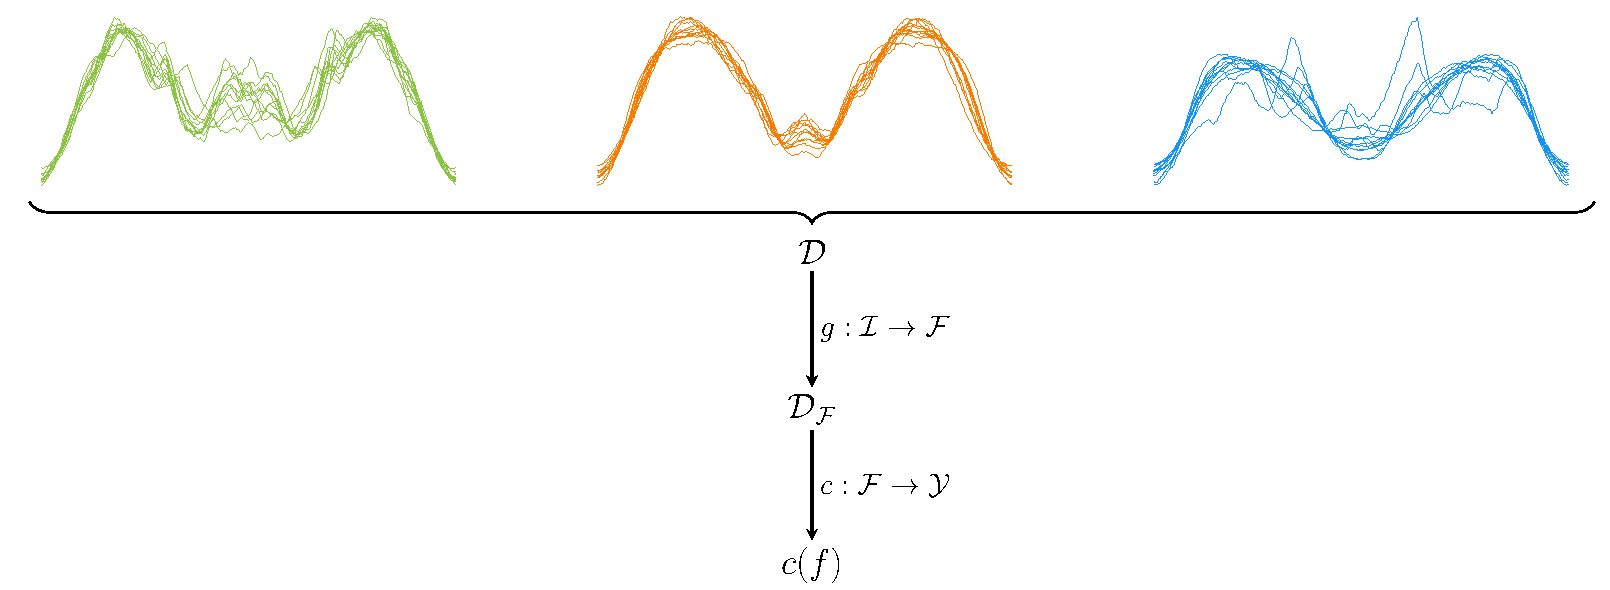
\includegraphics[width=1.1\textwidth]{timeseries.pdf}};
	        
	        \node[inner sep=0pt] (hist) at (0.07,-4.7)
	        {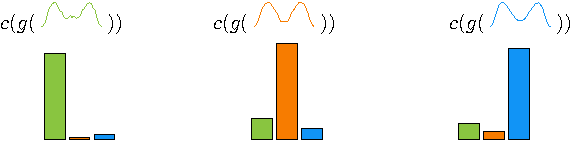
\includegraphics[width=.8\textwidth]{histograms.pdf}};
			
			\draw[-stealth, thick] ($(ts.south)+ (0.07, 0)$) -- node {} +(0, -0.8);				
			\draw[-stealth, thick] ($(ts.south)+ (0.07, 0)$) -- node {} +(-2.6, -0.8);
			\draw[-stealth, thick] ($(ts.south)+ (0.07, 0)$) -- node {} +(2.6, -0.8);
			
    \end{tikzpicture}
\end{document}